\chapter{$H_\infty$制御器設計の詳細}
$H_\infty$制御器設計の詳細な過程について述べる.
\section{伝達関数から状態空間への変換}
\label{sec:tf2ss}
油圧システムのバルブへの入力から出力までの伝達関数は\eqnname\eqref{eq:tf_in2fmsr}より,
\begin{align}
    \GinTofmsr = \frac{41.82}{(s+0.34)(s+130)}\mathrm{e}^{-0.016s}
\end{align}
である.
この伝達関数から状態空間への変換は一意ではないが,本研究においては「バルブへの指令電圧から推力まで」と「推力から出力まで」の2つのモデルの直列結合として表す.
前者の伝達関数モデルは\eqnname\eqref{eq:tf_in2fthr}より,
\begin{equation}
	\frac{3.4}{s+0.34}\mathrm{e}^{-0.01s}
\end{equation}
となるのでこの状態空間は
\begin{align}
	\begin{cases}
		\dot{x}_1(t) = -0.34x_1(t)+u(t-0.01) &\\
		y_1(t) = 3.4x_1(t)&
	\end{cases}
	\label{eqn:ss_inputTOfthr}
\end{align}
と表せる.
同様に,後者の伝達関数は
\begin{equation}
	\frac{123}{s+130}\mathrm{e}^{-0.006s}
\end{equation}
であるので,その状態空間は,
\begin{align}
	\begin{cases}
		\dot{x}_2(t) = -130x_1(t)+u_2(t-0.006) &\\
		y_2(t) = 123x_2(t)&
	\end{cases}
	\label{eqn:ss_ftheTOfmea}
\end{align}
となる.
よって式\eqref{eqn:ss_inputTOfthr}と式\eqref{eqn:ss_ftheTOfmea}の直列結合は,
\begin{align}
	\begin{cases}
		&\begin{bmatrix}
			\dot{x}_1(t-0.006)\\
			\dot{x}_2(t)
		\end{bmatrix}
		=
		\begin{bmatrix}
			-0.34 & 0\\
			1 & 0
		\end{bmatrix}
		\begin{bmatrix}
			x_1(t-0.006)\\
			x_2(t)
		\end{bmatrix}
		+
		\begin{bmatrix}
			3.4\\
			0
		\end{bmatrix}
		u(t-0.016) \\[10pt]
		&y =
		\begin{bmatrix}	
			0 & 123
		\end{bmatrix}
		\begin{bmatrix}
			x_1(t-0.006)\\
			x_2(t)
		\end{bmatrix}		
	\end{cases}
	\label{eqn:ss_inputTOfmea}
\end{align}
と表される.

\section{$H_\infty$制御器設計過程}
\label{sec:Hinfty_sekkei}
例として,むだ時間を無視した場合のコントローラ$K_{H_\infty}\mathrm{servo}$の設計過程を示す.
\subsection{乗法的摂動の見積もり}
$H_\infty$制御器設計の設計にあたっては,対象としているモデルの乗法的摂動を見積もる必要がある.
実対象制御モデルを$P_\mathrm{true}(j\omega)$,そのノミナルモデルを$P_\mathrm{nomi}(j\omega)$としたとき,
\begin{align}
    P_\mathrm{true}(j\omega)= (1+\Delta_m(j\omega))P_\mathrm{nomi}(j\omega)
\end{align}
で表される$\Delta_m(j\omega)$を乗法的摂動という.
ノミナルモデル$P_\mathrm{nomi}(j\omega)$はむだ時間を無視した場合のモデルである.
ノミナルモデルの周波数応答と,実制御対象の周波数応答\figname\ref{fig:crop-1018_manubode_in2fmea_7MPa}から乗法的摂動を求めると\figname\ref{fig:Wmanddeltam-crop}の赤丸のようになる.
この乗法的摂動を覆うように伝達関数$W_m$を決定すると,
\begin{align}
    W_m = 15\frac{s+10}{s+400}
\end{align}
となる.
$W_m$の周波数応答を\figname\ref{fig:Wmanddeltam-crop}に青実線で示す.
\figname\ref{fig4:konngoukanndo}において$W_T=W_m$とすることで,ロバスト性が保証される\cite{平田201703}.

\begin{figure}[t]
    \centering
        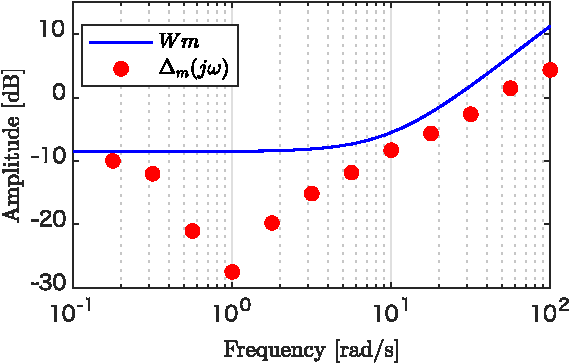
\includegraphics[keepaspectratio, scale=1.0]{contents/Appendix_Hinfty/figure/Wmanddeltam-crop.pdf}
        \caption{Multiplicative Perturbation}
        \label{fig:Wmanddeltam-crop}
\end{figure}

次に$W_S$を選ぶ.
$|W_S|$の逆数が感度関数$|S|$を覆うので,$1/|W_S|$が低周波領域で十分小さくなるように選ぶと$S$も小さくなり,目標値追従特性や外乱抑制が高まる.
これを考慮して,
\begin{align}
    W_S = \frac{5}{s+0.1}
\end{align}
とした.

$\varepsilon$は$w_1$から$y$までの直達項が0にならないようにするため入れる入力であり,$\varepsilon = 1e-3$とした.
これは観測ノイズと捉えることも可能である.

以上の設定の元に,$\gamma$イタレーションにより$H_\infty$制御器$\bar{K}_{H_\infty}\mathrm{servo}$を求めると,
\begin{align}
    \dot{x} & =
    \begin{bmatrix}
        -0.34&-1102270.49&461.19&-421.88\\
        1&-1664.57&0&0\\
        0&-648638.69&271.19&-248.17\\
        0&0&311.87&-285.06
    \end{bmatrix}
    x+
    \begin{bmatrix}
        8961.55\\12.48\\5273.49\\0
    \end{bmatrix}
    u           \\
    y       & =
    \begin{bmatrix}
        0&0&4.87&1.80
    \end{bmatrix}
    x
\end{align}
となる.
これに\ref{sec:サーボ系H無限大制御器}で示した積分器を結合させたのが,むだ時間を無視した場合のサーボ系$H_\infty$制御器$K_{H_\infty}\mathrm{servo}$となり,混合感度問題のゲイン線図は\figname\ref{fig:HinftyController-crop}となる.
\begin{figure}[t]
    \centering
        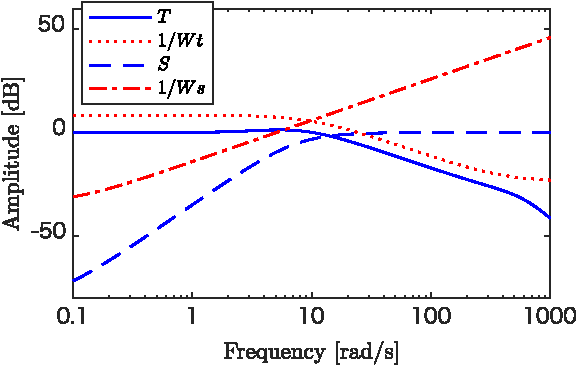
\includegraphics[keepaspectratio, scale=1.0]{contents/Appendix_Hinfty/figure/HinftyController-crop.pdf}
        \caption{Gain Graph of Mixed $H_\infty$ Problem}
        \label{fig:HinftyController-crop}
\end{figure}

また,むだ時間をPad\'e近似した場合のコントローラは
\begin{align}
    \dot{x} & =
    \begin{bmatrix}
        -255.34&6606.82&-105231.24&197.07&-209.83\\
        128&14740.75&-230324.2&0&0\\
        0&1055.90&-16373.36&0&0\\
        0&13213.12&-206454.94&49.17&-52.46\\
        0&0&0&61.79&-63.92
    \end{bmatrix}
    x+
    \begin{bmatrix}
    16489.91\\36094.04\\2565.87\\32353.49\\0
    \end{bmatrix}
    u           \\
    y       & =
    \begin{bmatrix}
    0&0&0&0.97&5.25
    \end{bmatrix}
    x
\end{align}
に積分器を結合したものである.